/F50/\\
\textbf{Prozess:} Gruppe verlassen\\
\textbf{Ziel:} ein Mitglied verlässt eine aktive Gruppe\\
\textbf{Kategorie:} primär
\textbf{Vorbedingung:} User ist Mitglied in einer aktiven Gruppe
\textbf{Nachbedingung (Erfolg):} User ist kein Mitglied mehr der aktiven Gruppe\\
\textbf{Nachbedingung (Fehlschlag):} User ist weiterhin Mitglied der aktiven Gruppe\\
\textbf{Akteure:} Gruppenmitglied\\
\textbf{Auslösendes Ereignis:} User möchte aus einer aktiven Gruppe austreten\\
1.) User entscheidet sich, aus der Gruppe auszutreten\\
2.) Er tippt auf den Namen der Gruppe und sieht die allgemeinen Informationen über die Gruppe (Namen, Mitglieder)\\
3.) Er tippt auf den Button "Gruppe verlassen"\\
4.) Ihm wird ein kleines Fenster im Vordergrund angezeigt, das ihn erneut fragt, ob er diese Gruppe wirklich verlassen will\\
5.a) Er tippt auf den Button "Ja, Gruppe verlassen"\\
5.b) Er tippt auf den Button "Nein, in der Gruppe bleiben"\\
6.a) Er wird zurück geleitet auf die Startansicht mit der Übersicht über die Gruppen. Dabei ist die gelöschte Gruppe nicht mehr mit aufgelistet.\\
6.b) Das kleine Fenster wird geschlossen und er kommt zurück zu Punkt 2)\\
7.a) Bei allen weiteren Gruppenmitgliedern wird der Name dieses Users nicht mehr in der Liste der Gruppenmitglieder aufgeführt\\

\begin{figure} [H]
	\centering
	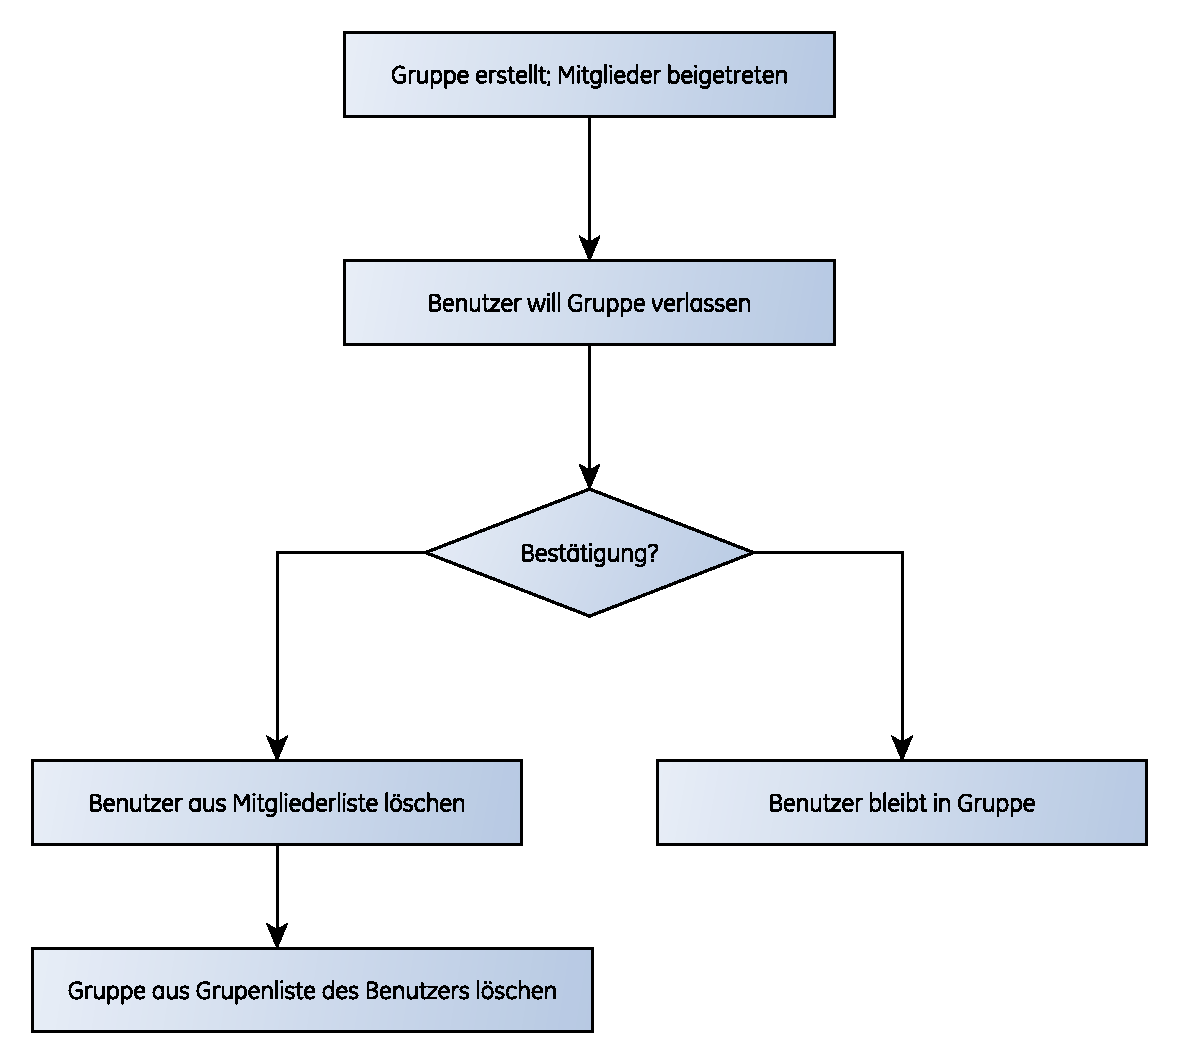
\includegraphics[scale=0.7]{./res/F50_gruppe_verlassen_flowgraph.pdf}
\end{figure}

